\documentclass[12pt]{article}
\usepackage{amsmath,amssymb,amsthm}
\usepackage{graphicx,mathabx}
\usepackage{xcolor}
\usepackage{tikz}
\usepackage{placeins}
\usepackage{lipsum}
\usepackage[shortlabels]{enumitem}
\begin{document}
\title{TCSS 343 - Week 2}
\author{Jake McKenzie}
\maketitle
\noindent\centerline{\textbf{Divide and Conquer}}\\\\\\\\\\\\\\\\
\begin{center}
``If anyone on the verge of action should judge himself according to the outcome, he would never begin." $~$ Søren Kierkegaard
\end{center}
\begin{center}
    ``A common mistake that people make when trying to design something completely foolproof is to underestimate the ingenuity of complete fools."
\end{center}
\begin{center}
$\sim$ Douglas Adams
\end{center}
\newpage
\noindent On the previous worksheet I had you write code for binary search. I want you to become more and more comfortable with trees and $\log{n}$ time. Work is just a function of ``How many problems we have" and ``the amount of work for each problem". Recursions trees is an extremely powerful way of illustrating the work of recurrence problems.\\\\
This will appear to be a digression but they are actually tightly connected ideas. Now remember the geometric series?
$$a + ar + ar^2+ar^3+\dots + ar^{n-1} = a\frac{1-r^n}{1-r}$$
Good, yeah I know who could have forgotten it!? It's one of my favourite series and it should be your best friend right about now.The geomtric series is a series which progresses by some multiplicative factor. \\\\
0. The first thing I will have you do is find $O(a\frac{1-r^n}{1-r})$ for two cases. When $r>1$ and $r<1$ where $a$ is some function of $n$.\\\\\\\\\\\\
\newpage
\noindent 1. Now that you've solved for those worst-case runtimes keep them for later because they're going to be useful! Now hold onto your butts because we're going to be having a lot of fun today. Complete this tree given the following recurrence for two more levels(The $a$ need not be the same as the previous $a$...sorry a habit of notation):\\
\centerline{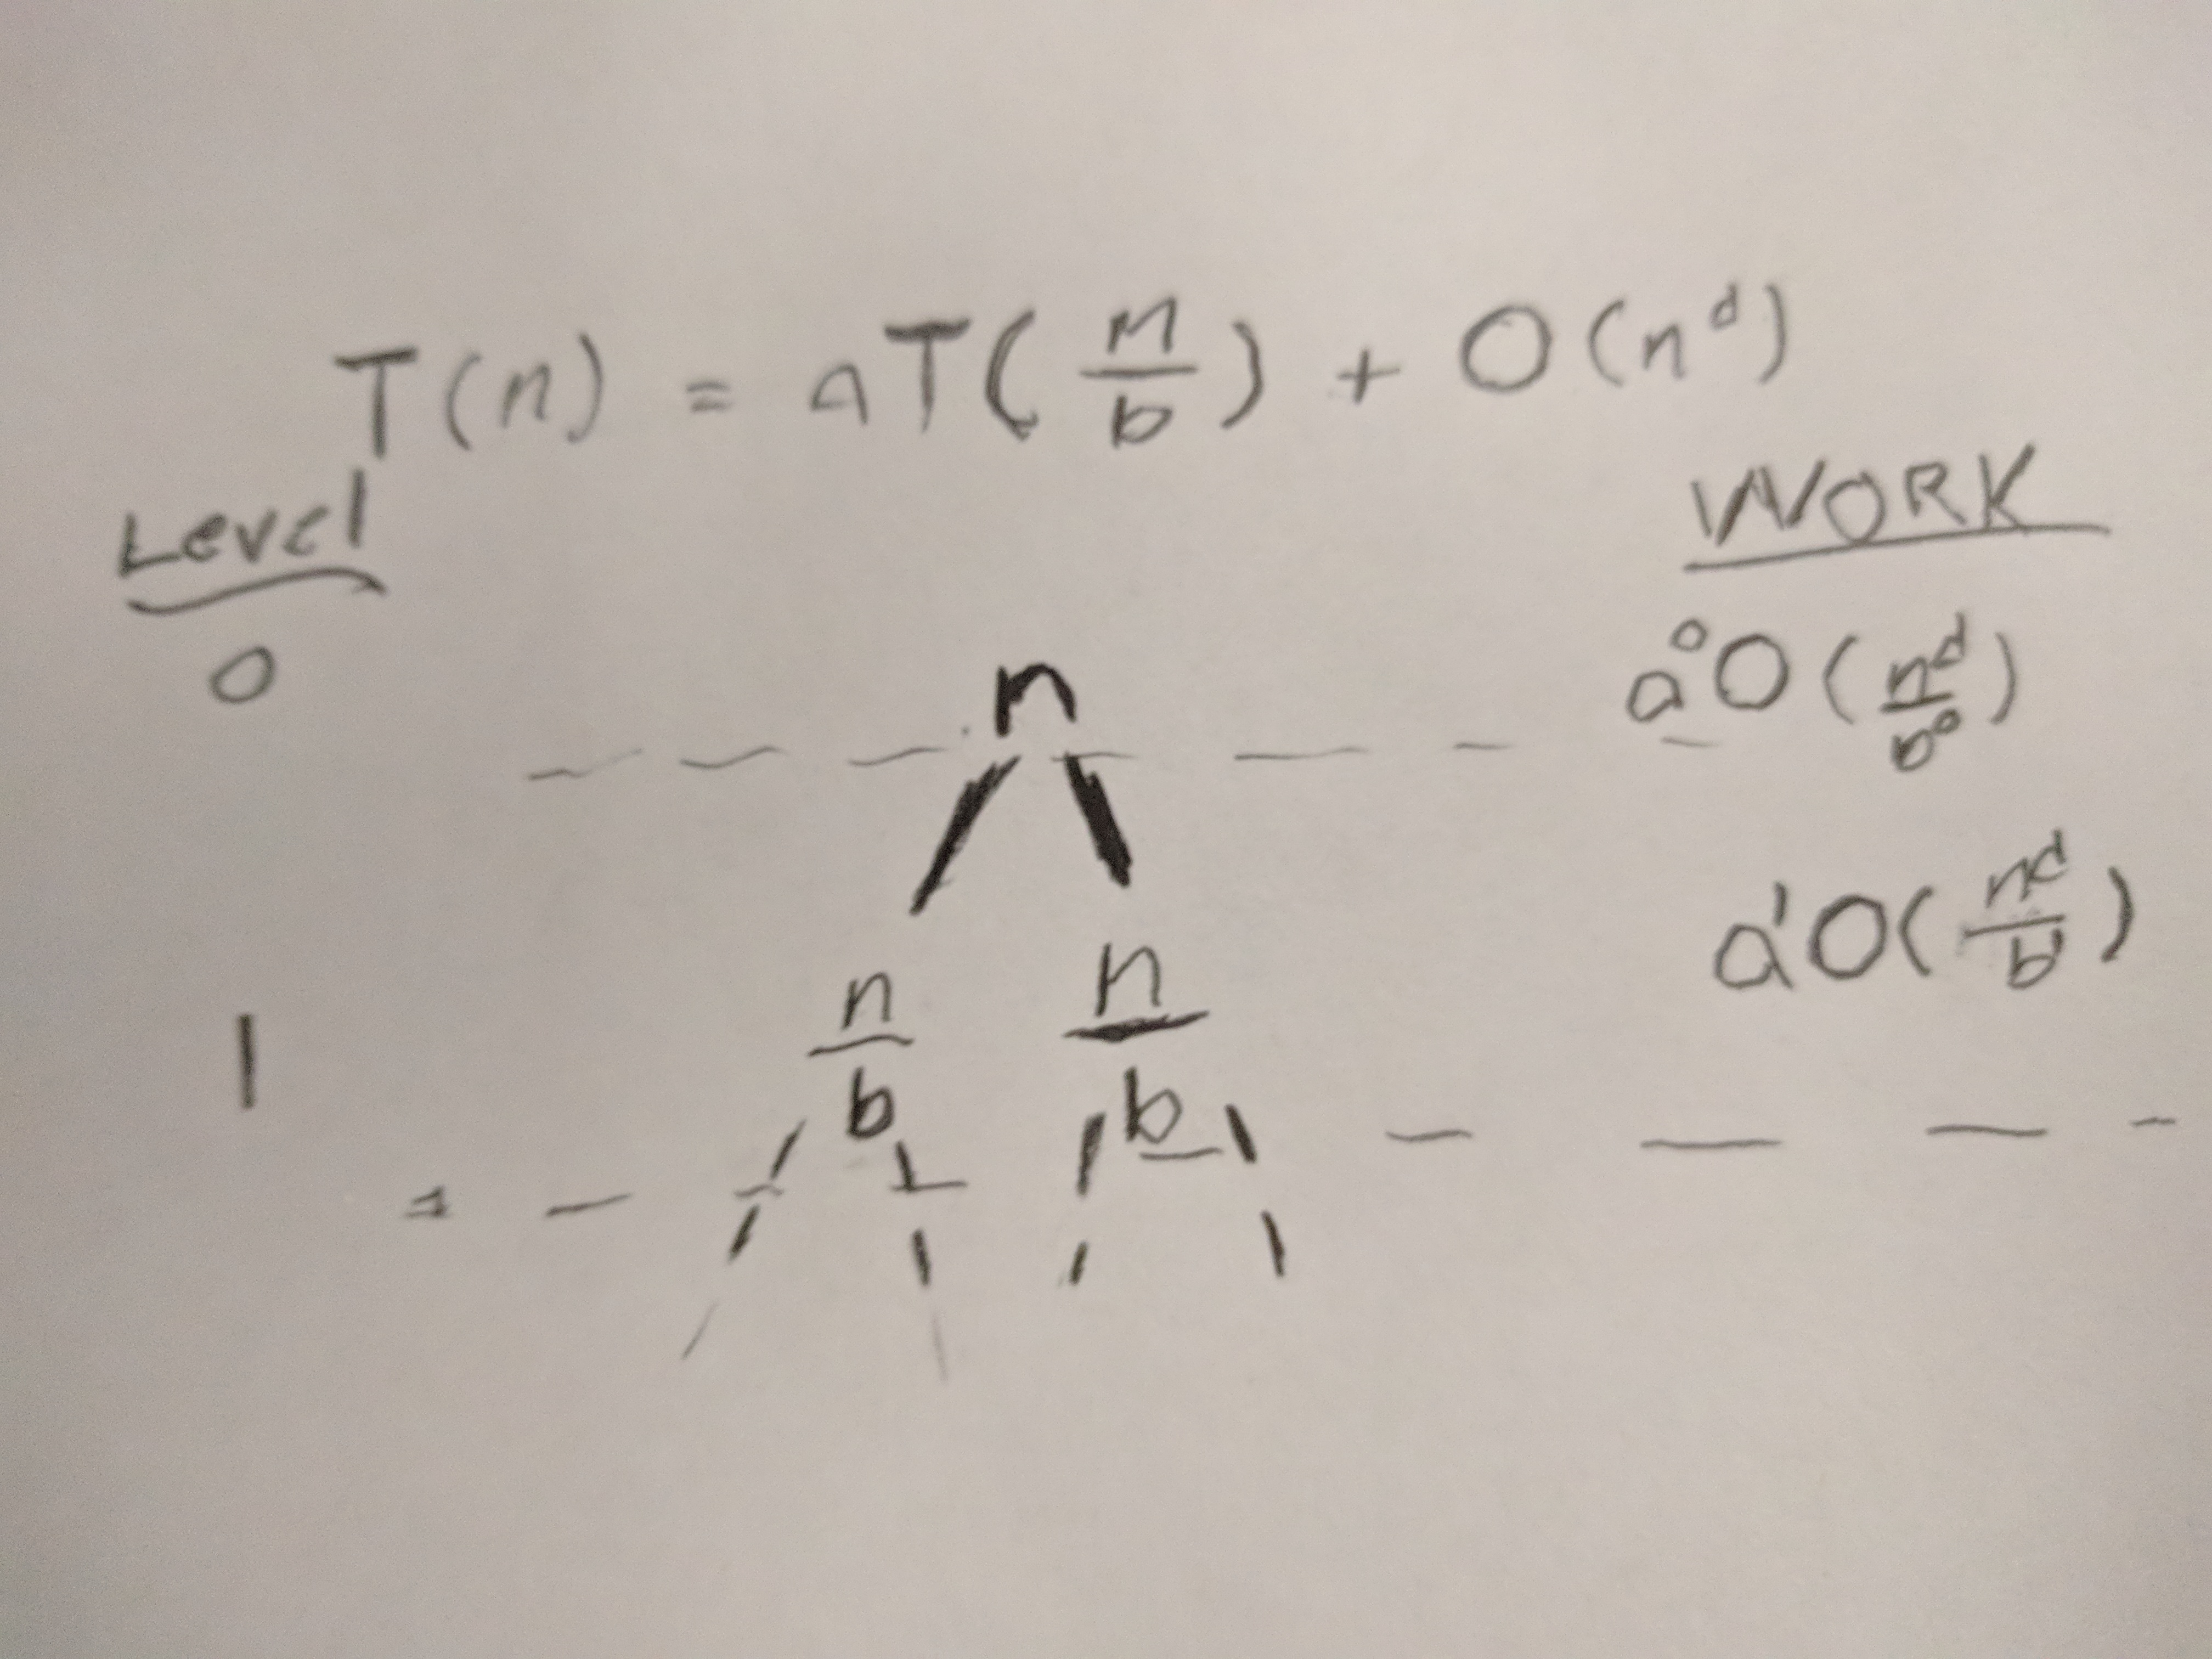
\includegraphics[scale = 0.05]{tree.jpg}} 
\newpage
\noindent 2. Take your previous result, at what level does the tree terminate?\\\\\\\\\\\\\\\\\\\\
3. Please, please try your darndest to express the total work as a summation. Remember: Work is just a function of ``How many problems we have" and ``the amount of work for each problem".
\newpage
\noindent 4. Solve for the three cases of the summation you found, when $r<1$, $r=1$ and $r>1$ find their worst case runtime. 
\newpage
\noindent 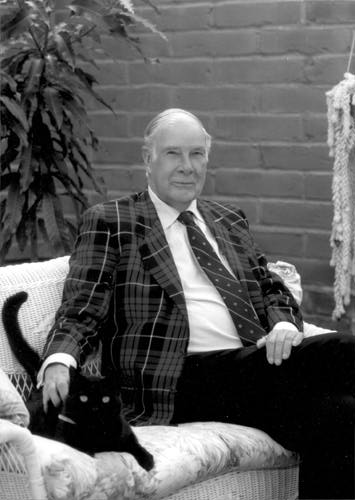
\includegraphics[scale = 0.2]{hamming_cat.jpg}\\
``The purpose of computing is insight, not numbers" - Richard Hamming\\\\
\noindent 5. Alright, alright I know...this isn't a math class this is an algorithms course! But if you solved those problems you now have a wonderful grab bag of results that you can use for now and forever! Now let's do some code.\\\\
Richard Hamming is one of my idols. He was a computer engineer who did a lot of really cool stuff and today we're going to calculate the distance that is named after him!\\\\
The Hamming distance between two integers is the number of positions at which the corresponding bits are different.\\\\
Given two integers $x$ and $y$, can you calculate this distance for me? Well...if not for me at least for Richard's cat.\\\\
\textbf{Note:}\\
$0 \leq x$,$y < 2^{31}$\\
\textbf{Example:}\\\\
\textbf{Input:} $x = 1$, $y = 4$\\\\
\textbf{Output: } $2$\\\\
\textbf{Explanation: }\\
\noindent 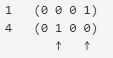
\includegraphics{hamming.jpg}\\
The above arrows point to positions where the corresponding bits are different(next page).\\\\
Write for me (or Richard's cat :3) some code to compute the hamming distance between two integers.
\newpage

\end{document}